\chapter{THEORETICAL BACKGROUND AND LITERATURE REVIEW}\label{intro}
\vspace{-3em}
This chapter explores previous works and approaches. It also discusses how modern techniques like image processing and machine learning are used for developing quick and smart identification and forecasting technologies. This chapter comes to an end with a critical appraisal that highlights the research gaps.

\section{Green View Index}


One of the indices available for quantifying roadside greening is the Green View Index (GVI). It was first proposed by \shortciteA{yang2009can}. The green view index (GVI) uses an observer's visual perception to quantify the urban space by simulating the pedestrian perspective of the road in street-view photo data and then calculating the percentage of vegetation in the road landscape. It is an effective way to acquire what people actually and typically see at street level on the ground. It is defined as the ratio of
the total green area from four pictures taken at a street intersection
to the total area of the four pictures, calculated using the following
equation:
\begin{equation}
\text{Green View} = \frac{\sum_{i=1}^{4} \text{Area}g_i}{\sum_{i=1}^{4} \text{Area}t_i} \times 100\%
\end{equation}
where $\text{Area}_{g_i}$ is the number of green pixels in the picture taken in
the ith direction among the four directions (north, east, south and
west) for one intersection, and $\text{Area}_{t_i}$ is the total pixel number of
the picture taken in the ith direction.

\shortciteA{li2015assessing} modified the GVI and used six images covering
the 360◦ horizontal surroundings to calculate the index for each
sample site along streets. The final modified GVI used calculated using 18 images for each site.
The modified GVI calculation formula is written as
\begin{equation}
\text{Green View} = \frac{\sum_{i=1}^{6} \sum_{j=1}^{3} \text{Areag}_{ij}}{\sum_{i=1}^{6} \sum_{j=1}^{3} \text{Areat}_{ij}} \times 100\%
\end{equation}
where $\text{Area}_{g_ij}$ is the number of green pixels in one of these images
captured in six directions with three vertical view angles (−45◦, 0◦,
45◦) for each sample site, and $\text{Area}_{t_ij}$ is the total pixel number in
one of the 18 images.

\section{Aerial Image}
An aerial image specifically refers to a photograph or digital image captured from an elevated perspective, typically obtained via drones or satellites. These images serve as crucial data inputs for analyzing and mapping various features, including land cover, vegetation, and environmental changes, facilitating the application of deep learning techniques for tasks such as green space identification and segmentation. Figure \ref{aerialimage} shows how aerial images differ from street-view images.
\begin{figure} [H]
\centering
% \vspace{-30mm}
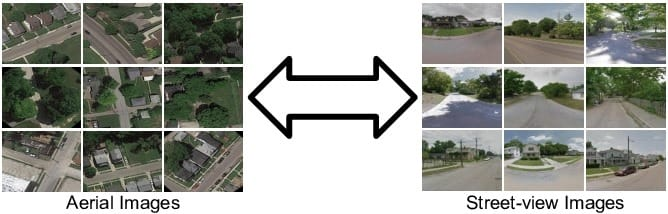
\includegraphics[width=1\textwidth, height=\textwidth,keepaspectratio]{figures/aerialimg.jpg}
% \vspace{-25mm}
\caption{Aerial Image vs Street-View Image}
\label{aerialimage}
\end{figure}
\section{Digital Image Processing}
Digital Image Processing (DIP) is the manipulation and analysis of images using computer algorithms. It involves enhancing, analyzing, and extracting information from digital images to improve their quality or extract meaningful data. Techniques like image enhancement, image restoration, object detection, image segmentation, and pattern recognition fall under DIP. 
\section{Semantic Segmentation}

Semantic segmentation is a type of deep learning system that gives each pixel in an image a label or category. It is used to distinguish between a set of pixels that belong to distinct categories \shortcite{chai2020aerial}. For example, an autonomous vehicle needs to be able to identify other vehicles, people, pavement, traffic signs, and other features of the path. Semantic segmentation is used in many applications such as automated driving, medical imaging, industrial inspection and object detection, etc.

A simple example of semantic segmentation is separating the images into two classes. For example, in Figure \ref{Semantic}, an image showing a person at the beach is paired with a version showing the image's pixels segmented into two separate classes: person and background.

\begin{figure}[H]
\centering
% \vspace{-30mm}
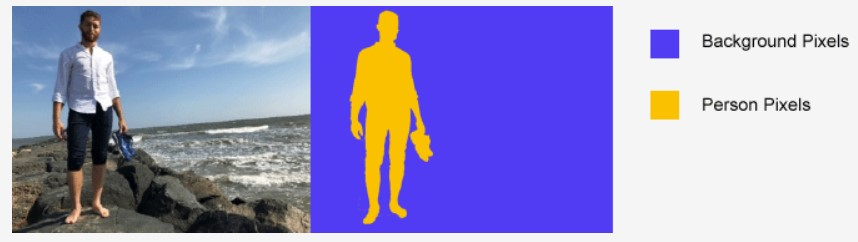
\includegraphics[width=1\textwidth, height=\textwidth,keepaspectratio]{figures/Semantic.jpg}
% \vspace{-25mm}
\caption{Semantic Segmentation}
\label{Semantic}
\end{figure}

\section{Machine Learning}
The goal of machine learning (ML) is to comprehend and develop "learning" techniques, or tactics that use data to improve performance on specific tasks. \shortcite{mitchell1997machine}. That's regarded as a part of artificial intelligence. Machine learning algorithms use sample data, also known as training data, to build a model using which they may make predictions or judgments without having to be taught \shortcite{sag2018new}. In many fields, such as computer vision, speech recognition, email filtering, health, and agriculture, where it is difficult or impractical to develop conventional algorithms that can complete the necessary tasks, machine learning algorithms are employed.
 \shortcite{hu2020voronoi,yoosefzadeh2021application}. Performing machine learning can involve creating a model, which is trained on some training data and then can process additional data to make predictions. The machine learning models used in this thesis fall under Deep Learning, which is a new field of study in machine learning. It is made up of several artificial neural network hidden layers. \shortcite{vargas2017deep}

\section{Deep Learning Architectures}
Deep Learning models are based on Artificial Neural Networks. These neural networks are inspired by the structure and function of the human brain’s biological neurons and are modeled to learn from a vast number of data. Due to the availability of enormous datasets and advancements in computing power, the popularity of Deep Learning has grown in recent years \shortcite{vargas2017deep} The deep learning architectures used in this thesis are described below.

\subsection{U-Net}
U-Net is a popular architecture in satellite image analysis. As shown in Figure \ref{U-Net} U-Net's architecture has two paths: a contracting road and an expanding method  \shortcite{singh2023semantic}. The expanding path contains decoder layers that decode the encoded data and use the information from the contracting path via skip connections to generate a segmentation map. The contracting path lowers the spatial resolution of the input and finds the relevant features in the supplied image. The encoder layers perform convolutional operations that reduce the spatial resolution of the feature maps while increasing their depth to capture increasingly abstract representations of the input. 
%On the other hand, the expanding path finds the features and decodes the encoded data without compromising the spatial resolution of the input. In the expanding route, the decoder layers perform convolutional operations in addition to upsampling the feature maps. The skip connections from the contracting path help the decoder layers locate the features more precisely by preserving the spatial information lost in the contracting path.

\begin{figure} [H]
\centering
% \vspace{-30mm}
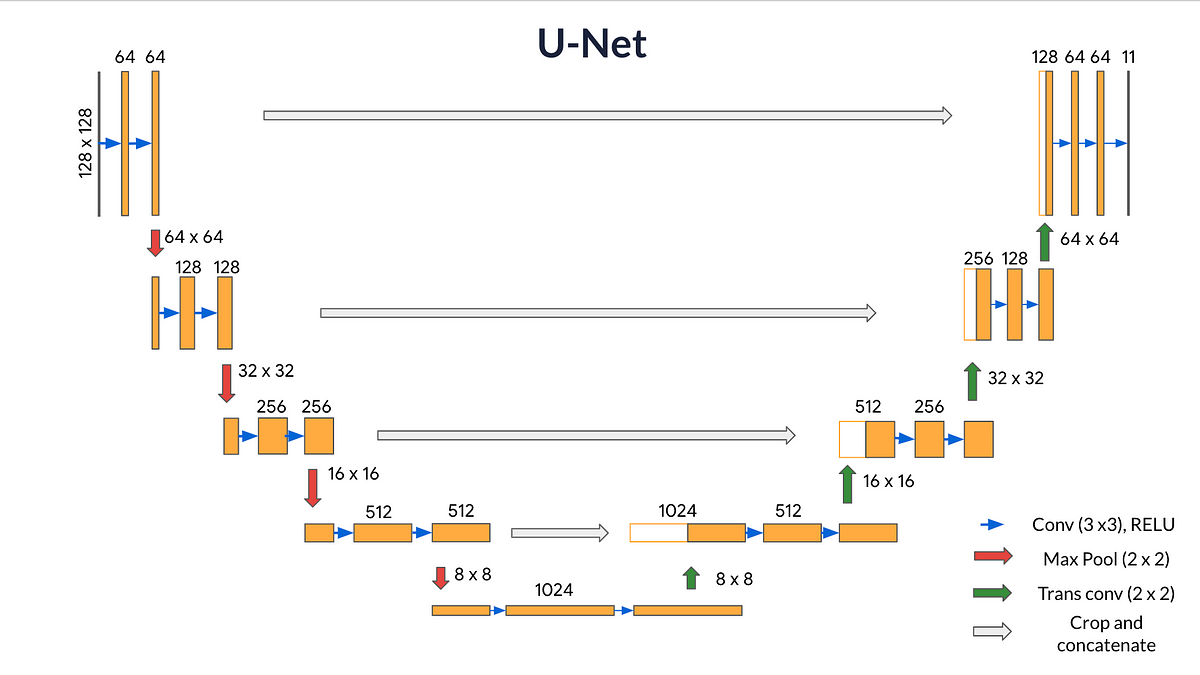
\includegraphics[width=1\textwidth, height=\textwidth,keepaspectratio]{figures/U-Net.png}
% \vspace{-25mm}
\caption{U-Net}
\label{U-Net}
\end{figure}
\subsection{SegNet}
This novel and practical deep fully convolutional neural network architecture for semantic pixel-wise segmentation was proposed by \shortciteA{segnet2}. As shown in Figure \ref{Segnet}, Segnet uses an encoder network and a corresponding decoder network comes before a pixel-wise classification layer. SegNet only requires forward evaluation of a fully learned function to obtain smooth label predictions. Additionally, a larger context is considered for pixel labeling which improves accuracy. Moreover, it is easy to visualize the effect of feature activation(s) in the pixel label space at any depth.\shortcite{segnet1}

\begin{figure} [H]
\centering
% \vspace{-30mm}
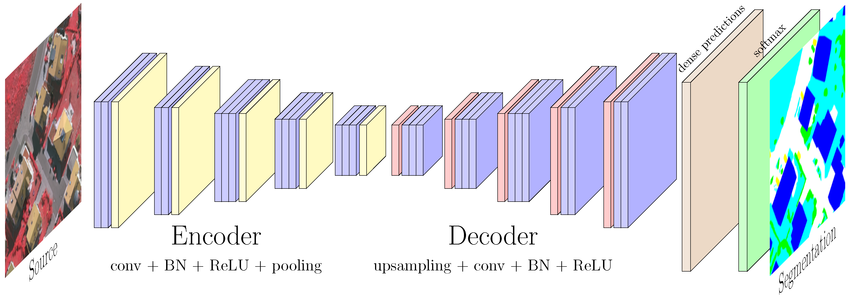
\includegraphics[width=1\textwidth, height=\textwidth, keepaspectratio]{figures/SegNet.png}
% \vspace{-25mm}
\caption{Segnet Architecture}
\label{Segnet}
\end{figure}
\subsection{DeepLabv3plus}
DeepLabV3plus is an advanced deep neural network architecture for semantic image segmentation which improves upon DeepLabV3 by integrating multi-scale feature fusion and Atrous Spatial Pyramid Pooling (ASPP) modules for better context understanding \shortcite{deeplab2}. Atrous Spatial Pyramid Pooling efficiently harvests multi-scale characteristics with valuable information for segmentation \shortcite{deeplab1}. As shown in Figure \ref{Deeplabv3}, the input image is encoded into a compressed representation using an encoder, and then these characteristics are upsampled to the required resolution using a decoder. With its encoder-decoder architecture and skip connections, it achieves high accuracy in segmenting objects of varying sizes. 
\begin{figure} []
\centering
% \vspace{-30mm}
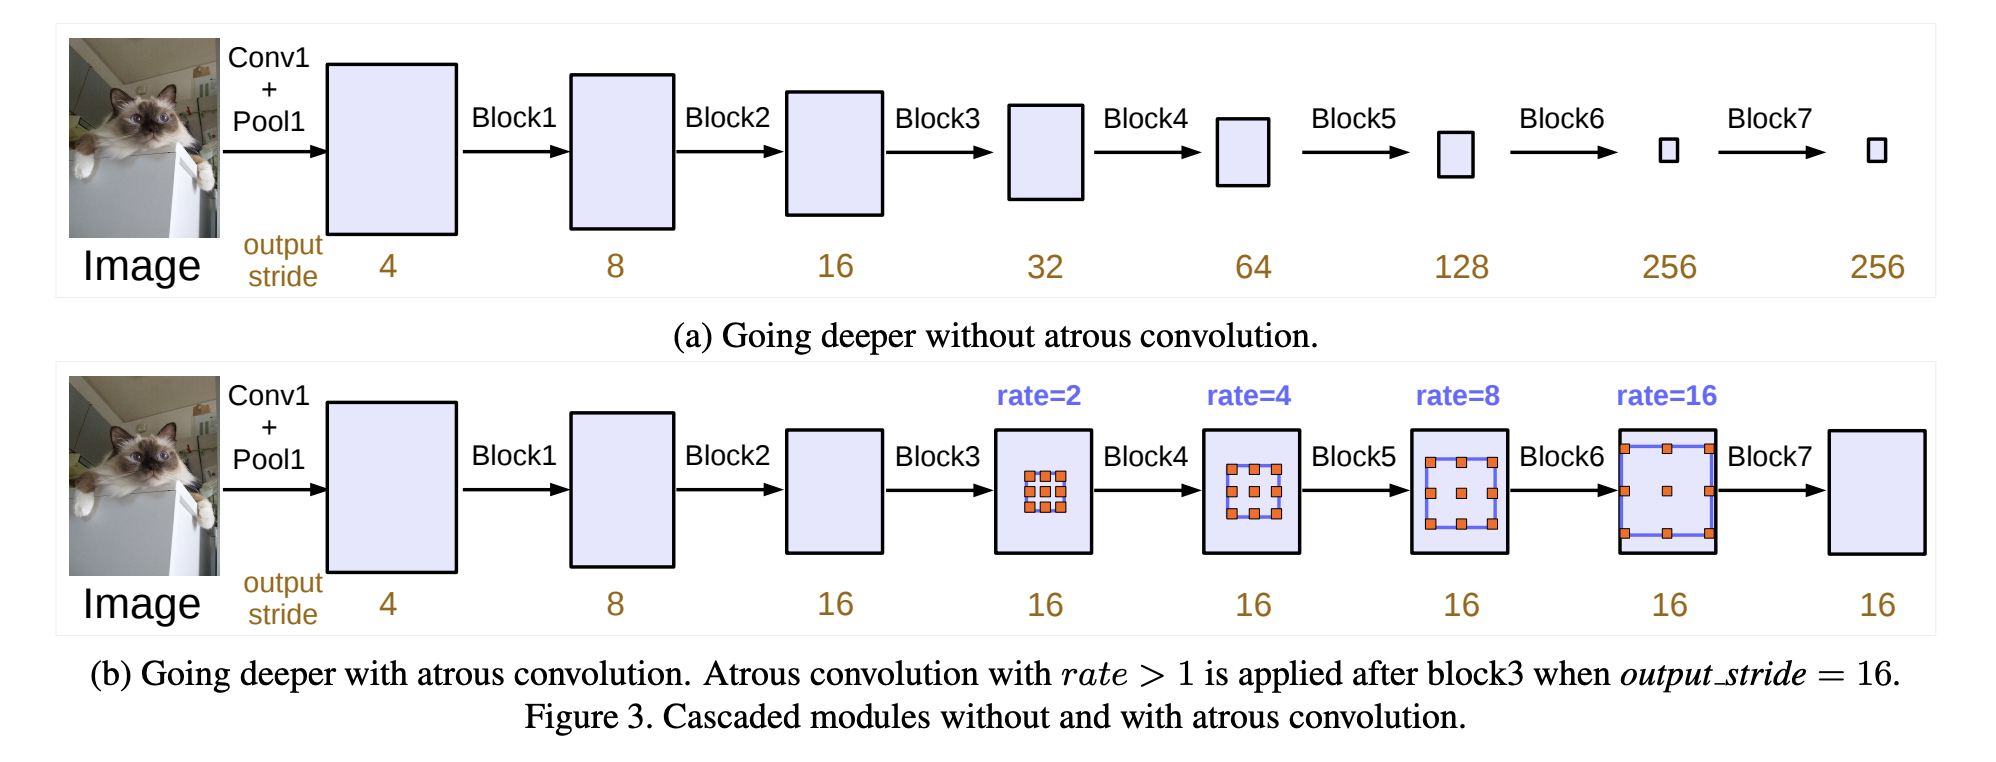
\includegraphics[width=1\textwidth, height=\textwidth,keepaspectratio]{figures/Deeplabv3.png}
% \vspace{-25mm}
\caption{Deeplabv3 Architecture}
\label{Deeplabv3}
\end{figure}
\section{Recurrent Neural Network}

    \sub
    RNN, or Recurrent Neural Network, is a class of neural networks specially designed for processing sequential data by maintaining an internal state or memory. Unlike feedforward neural networks, which process data in a single direction, RNNs have connections that loop back, allowing them to exhibit temporal dynamics and learn patterns over time. RNNs are widely used in tasks such as language modeling, speech recognition, and time series prediction.
    RNN has variants like LSTM and GRU. 
    \subsection{LSTM (Long Short-Term Memory)}
    Long Short-Term Memory is a type of computer algorithm used for processing sequences of data, like sentences or time-series data. It's special because it can remember important information for a long time while also quickly forgetting irrelevant details. This makes it great for understanding and predicting patterns in sequences, such as in natural language processing tasks like language translation or sentiment analysis \shortcite{lstm}
    
   

    \subsection{GRU (Gated Recurrent Unit)}
    Gated Recurrent Unit, is a type of recurrent neural network (RNN) architecture designed to address the vanishing gradient problem encountered in traditional RNNs. GRU incorporates gating mechanisms to regulate the flow of information through the network, allowing it to retain long-term dependencies more effectively. With fewer parameters compared to other RNN variants like LSTM (Long Short-Term Memory), GRU offers computational efficiency while achieving comparable performance in sequence modeling tasks such as natural language processing and time series prediction. \shortcite{gru}

     \subsection{Siamese Neural Network Model}
    A Siamese model is a neural network architecture designed for comparing similarity between pairs of inputs. It consists of two identical subnetworks (or twins) that share the same weights and architecture. Each input is processed independently by one of the subnetworks, and the outputs are then compared using a distance metric. Siamese Neural Networks are a type of neural network design consisting of two or more identical subnetworks. In this case, "identical" means that their weights and parameters are the same. The parameter updates are mimicked by the two sub-networks. Because these networks can compare feature vectors to ascertain how similar the inputs are, they are helpful in a wide range of applications \shortcite{siamese}. Siamese models are commonly used in tasks like image recognition, signature verification, and similarity-based recommendation systems.
   




%\section{Visual Search and Recommendation of Products}

%\cite{12_lit} worked on a visual search engine architecture using deep learning and machine learning techniques, with a proof-of-concept implementation focusing on the fashion e- retail industry. It first classifies the query image to the right category using image classification. Then all the images in that category are ranked based on their similarity and the top images are retrieved as recommendations. In the category prediction phase for various DNN models, CNN gives the highest accuracy of 83\% with much less training time when compared with other models. MobileNet results in much higher accuracy, giving a precision of 70\%, and the least latency time of all DNN models. Thus they chose MobileNet as the training model in the enhanced ViSeR implementation combined with the SGD classifier. For the image similarity module, they adopted the approach of cosine distance in the final proof-of-concept model. \cite{13_lit} implemented a system that will scan real-time world objects and identify them based on the deep learning algorithm. There are three phases for the searching technique: scanning, detection, and recommendation. With the help of YOLO(deep learning object recognition technique), the image of the object will be scanned, once the object is detected it will recommend the desired product to the customer/user using web mining. A system that helps users search for the product and its surrounding suppliers with the image of the product they want, thereby making it easier to order the product was proposed by [\cite{14_lit}]. They made sure to search for the desired product well by enabling a highly accurate image search with pre-processing and inpainting. 

 \section{Related Works}

 The existing research works have been divided into four sections: measuring green space, segmenting green space from images, analyzing change in land and predicting change in land coverage. There are two categories for segmentation works: segmentation with Google Street View photos and segmentation using aerial images. This section has studied, analyzed, and discussed existing works. 

\subsection{Measuring Green Space from Images}
 \shortciteA{yang2009can} proposed a new index called Green View (GV) in their paper that measures the amount of greenery that people can see on the ground at different locations in a city. The researchers tested the Green View index in Berkeley, California. Their research combines field surveys and photography interpretation.
%Land cover information was derived from aerial photographs and classified using an object-based image analysis approach.%
The image was first segmented into image objects using a
multi-resolution segmentation algorithm. After segmentation, an
iterative classification process was run to classify image objects
into land cover classes until the classification results could not be
improved by more iteration. Six land cover classes were identified and the accuracy of the classification
result was determined by using a reference data set which are patches
of different land cover types identified from the image and verified
on the ground.
Green View was measured using a two-step process.
Sampling sites were selected based on a random sampling approach using a street map.
Secondly, 
pictures were taken at selected intersections in four directions.
Green vegetation areas in pictures were quantified by counting green pixels. 
The green view index was computed by manually extracting only the green pixels using Adobe Photoshop for the image and then the ratio of green pixels over total pixels was calculated. 
Green View values were calculated for each intersection and averaged for each census tract.
Overall Green View for Berkeley was determined by weighting values based on the number of intersections in each tract.
The authors successfully concluded that the overall Green View value of their subject location was 24.79\%, indicating the visibility of urban forests.
%Moreover, the green view index strongly correlated with the canopy cover of trees and shrubs, which was 31.49\%.
%The authors suggested that the use of Green View can be expanded to evaluate the visual impact of various planning and management practices on urban forests. Future studies may apply the Green View index to other cities and regions to assess their urban forests' visibility.
\newline
Based on the previous research, \shortciteA{li2015assessing} modified the existing Green View Index (GVI) formula and conducted a case study assessment of street greenery using GSV images in the area of East Village, Manhattan District, New York City. They explored Google Street View (GSV) as a street-level, urban greenery assessment tool. 
They used 18 GSV images from different angles to create a more objective measurement. This covers a 360° horizontal view and 180° vertical profile, offering a comprehensive assessment of street greenery.
From the images, green vegetation was extracted using the difference of Green band from Red and Blue band. An additional rule
that pixel values in green band must be larger than those in the red band. 
The green vegetation extraction results were then compared with manually extracted green vegetation for the same image using Adobe Photoshop. \newline
In another study, \shortciteA{li2018mapping} also utilized Google Street View (GSV) and remote sensing data to estimate street tree shade provision in Boston during the leaf-on season. Using the sky view factor (SVF) to quantify shade, the research mapped the spatial distribution and results found that street trees contribute 24.6\% of shade citywide, with the southwestern part exhibiting the highest coverage.
 From their research, the authors concluded that GSV images
are qualified for assessing street greenery and the modified GVI may be a more objective measurement of street-level greenery. However, using GSV images has some limitations that include time inconsistency and coverage of a limited number of viewing points.
\newline
Similarly, \shortciteA{degerickx2017mapping} acquired a hyperspectral dataset of Brussels and created a spectral library which was used to classify the urban green types in the hyperspectral imagery through a spectral angle mapper algorithm. The study successfully identified and classified various types of urban green areas in Brussels with high accuracy. \newline
\shortciteA{berland2017google} explored the use of Google Street View (GSV) for virtual street tree surveys in municipal forestry. The research indicated GSV's potential for reliable genus identification and compared GSV data with field survey results, emphasizing GSV's promise as a geospatial tool for urban forestry research.
\newline
\shortciteA{richards2017quantifying} also used Google Street View images to analyze and quantify green canopy coverage along Singapore's road network. Results showed that trees shaded 13\% of annual solar radiation, with notable variations across urban land-use types, and showcased a correlation between human and machine estimates of canopy cover.

In another similar work, \shortciteA{changeinland7} assessed street greenery using three indicators: Green View Index (GVI), Normalized Difference Vegetation Index (NDVI), and newly introduced Vegetation Structural Diversity (VSD). To gather data on street greenery in the urban area of Nanjing, China they have utilized street view images and satellite images. A semantic segmentation method was applied to extract GVI and VSD from street view images, while NDVI was calculated using satellite images. It also compared overhead greenery and eye-level greenery based on different Urban Functional Zones (UFZs) such as residential, open spaces and industrial lands. They also made a comparison on how the indicators perform in new city vs old city. The findings from their research suggests that indicators of street greenery  can provide a comprehensive reference for building more
human-friendly and diversified street green belt.


\subsection{Segmentation using Machine Learning approach}

\subsubsection{Using Google Street View image}
\shortciteA{cai2018treepedia} applied state-of-the-art deep learning models,
and compared their performance to a previously established
benchmark of an unsupervised method. They also trained
a DCNN end-to-end model that directly estimates GVI in
GSV images. 
To validate accuracy in estimating GVI, 
the authors used 100 labeled GSV images and calculated Pearson’s correlation coefficient between GVI from labeled images
and model estimates.
%Additionally, they proposed two additional metrics to validate
%the prediction accuracy of their models: Mean Intersection over-Union and Mean AbsoluteError. 
%By using street-level GSV images, it is possible to utilize
%the abundance of open-source manually labeled street-level
%image datasets to heavily pre-train the DCNN models. After
%pre-training, they tuned the DCNN models to GSV images
%by training on a small-scale dataset. This saves significant
%resources that would normally be associated with building
%a large custom training dataset. 
By using street-level GSV images and DCNN models, researchers can utilize
vast street-level image datasets to learn and understand
complex environmental and socio-economic phenomena,
in addition to urban tree cover. \newline
Similarly, \shortciteA{seiferling2017green} used Google Street View images of New York and Boston to segment and quantify the percentage of tree cover in streetscape images using a multi-step
computer vision algorithm. By modeling the relationship between neighboring images along city street segments,
the authors successfully estimated the amount of perceived tree cover in the city
streetscapes to a relatively high level of accuracy.

\subsubsection{Using Satellite Images}
\shortciteA{chen2022enhanced}  created a neighborhood-scale
urban community green space (UCGS) dataset and proposed a segmentation decoder with
two auxiliary branches for HRNet. Their proposed model added
two additional branches to the low-resolution representations 
to improve their discriminative ability,
thus enhancing the overall performance when the high- and low-resolution representations are fused.
To evaluate the performance of the model, it was tested on a dataset that includes satellite images
of Shanghai, China.
Pixel-based
categorization approaches such as Maximum Likelihood (ML) and Random Forest (RF) were also used to compare the proposed model's performance.
The precision, recall, F1-score, IoU, and Overall Accuracy of all the approaches were compared. The proposed model showed the most accurate
UCGS detection accuracy among all comparison models. In particular, it achieved a great
improvement in the identification of green spaces covered by shadows.\newline 
On the other hand, \shortciteA{demir2018deepglobe} addressed three different tasks which included land classification from satellite images using semantic segmentation. For the tasks, they created a dataset of 10,000 satellite images.
They performed pixel-wise classification on their data by designing a CNN architecture based on DeepLab using ResNet18 backbone with
atrous spatial pyramid pooling (ASPP) block and batch normalization. Data augmentation was performed by integrating rotations and also weighted classes based on class distributions.
This approach achieved an IoU score of 0.433 %at epoch 30 with a 512×512 patch size.
Their work contains some challenges in classification including distinguishing between small structures not annotated in the ground truth and handling harder distinctions between land cover classes.

\subsection{Analysis of Change in Land}

\shortciteA{changeinland6}  developed a deep mapping approach using a Siamese Convolutional Neural Network (SCNN) to detect visual changes indicative of gentrification in urban areas, focusing specifically on individual properties in Ottawa, Canada. They utilized temporal sequences of Google Street View (GSV) images to track improvements in frontage quality over time. By employing the SCNN, they achieved a high test accuracy of 95.6\% in detecting gentrification-like visual changes. The researchers were able to identify the precise places and periods when gentrification processes were taking place in the study area. Insights into the spatial distribution of gentrification processes were obtained by the mapping of spatial concentrations of visual property improvements made easier by the application of Kernel Density Estimation (KDE). 
 %The study identifies visual indicators of gentrification, it does not directly account for socioeconomic or cultural changes within the neighborhoods studies. The performance of the SCNN model may be influenced by the quality and representation of the training dataset.

 In the same way, \shortciteA{changeinland5} conducted a study on gentrification in the Canadian city of Toronto, exploring its coevolution in both residential and non-residential sectors. They combined multiple data sources to analyze gentrification patterns, including household income, educational attainment, building permits, and establishment compositions. To characterize spatial units based on a composite measure of the gentrification process they employed mas-p-regions clustering. A Bayesian hierarchical spatial (BHS) model was developed to describe changes in residential property prices over five years. Their research offered an in-depth discussion of the causes and defining characteristics of gentrification, as well as insights into the coevolution of the phenomenon in both the residential and non-residential sectors.

 

 
 \shortciteA{changeinland2} analyzed annual forest loss data from the University of Maryland and Global Forest Watch. They used different confidence levels to distinguish between forest loss which is caused directly by fire and other causes like deforestation or natural events. A baseline of areas was established with > 30\% tree coverage density in 2000 and primary forest loss was identified. %by intersecting forest cover loss data with a dataset of primary humid tropical forests. 
They successfully identified deforestation hotspots by conducting a kernel density estimate analysis, which calculates the magnitude per unit area of the forest cover loss, using different parameters and tools.
%such as the kernel Density tool from the Spatial Analyst Tool Box of ArcGIS. 
%However, the geographic range for the analysis was designed for maximum inclusion but may not capture all relevant areas or factors contributing to deforestation in the Amazon region.
\newline
In another work, \shortciteA{changeinland3} utilized Convolutional Neural Networks (CNNs) to analyze high-resolution RGB imagery captured by Unmanned Aerial Vehicles (UAVs) for mapping vegetation cover and species distribution. A straightforward CNN architecture was employed. Mapping tree species cover in primary forests, identifying plant invasions by woody species, and mapping vegetation succession in a glacier foreland are the main focus of their research. They achieved commendable accuracies across all case studies, with the accuracy increasing with larger tile sizes, capturing a broader spatial context. Moreoever, they demonstrated the efficacy of CNNs in harnessing high-resolution data from UAVs to map vegetation patterns accurately.


\shortciteA{nawar2022present} have utilized UAV technology and convolution Neural Networks (CNNs) to map vegetation patterns in Dhaka city. The research formulated to calculate changes in Green spaces in Dhaka City between 1989 and 2020 using GIS and Remote Sensing techniques. 
Using remote sensing techniques, classification and NDVI methods of satellite imagery, they have found a drastic reduction in green spaces over the past three decades, particularly healthy vegetation, alongside urban infrastructure expansion.

 %Howver, the quality of the input data, determines how accurate and dependable the findings are. Moreoever, the CA-Markov model used  oversimplifies complicated urban dynamics and may miss important elements that affect UGS loss.


%The method's reliance on low-cost RGB sensors makes it accessible to a wide range of users, indicating its potential for ecological applications. However, due to low resolution of their dataset, their work was unable to differentiate between finer details of plant canopies.
\subsection{Predicting Change in Land Coverage}


\shortciteA{changeinland8} used a hybrid model called the Multi-Layer Perceptron-Markov Chain (MLP-MC) to study changes in land use and land cover (LULC) in regions of Saudi Arabia from 1990 to 2018 and then predict future scenarios for 2040. The authors collected Landsat satellite images for 1990, 2000, and 2018, and used a Maximum Likelihood Classifier (MLC) algorithm to classify the images into different land cover classes. To evaluate the accuracy of these classified maps, a cross-classification method and field surveys were utilized. For predicting future changes, the Markov Chain analysis was applied to estimate transition matrices for different years, calculating LULC transition potential maps. The accuracy of their predictions was validated using measures like overall accuracy, kappa coefficient, Land Absorption Coefficient (LAC), and Land Consumption Rate (LCR). The overall classification accuracy for the years 1990, 2000, and 2018 ranged from 88.40\% to 91.21\%, with corresponding kappa coefficients indicating satisfactory accuracy.

Similarly, \shortciteA{changeinland9} studied how population growth and migration in the lower Himalayan regions of Pakistan led to urbanization, changing land use and increasing land surface temperature (LST) from 1990 to 2017. They used Landsat data and the support vector machine (SVM) method to analyze these changes. For predicting future trends in 2032 and 2047, they developed a model called CA-ANN, combining cellular automata and artificial neural network, using data from 2002 and 2017, achieving a correctness value of 70\% .

In another study, authors \shortciteA{changeinland10} studied how land cover (like forests and fields) changed in the Javadi Hills, India, between 2009 and 2015. They used satellite images from 2009, 2012, and 2015 and classified the images using Random Forest Classification to see how the land cover changed. Next, they compared two different models, the Markov chain–artificial neural network with cellular automata (MC–ANN–CA) and Markov chain–logistic
regression with cellular automata (MC–LR–CA) to predict how the land cover might change in 2021 and 2027. They also considered factors like slope, elevation, and distance to roads to help with their predictions. Finally, they compared their predictions to real data from 2015 to see how accurate they were. The research found that the combination of artificial neural network and cellular automata was more accurate (correctness of 93.68\% and the kappa
value of 0.85).

Likewise, \shortciteA{changeinland1} aimed to assess urban green space (UGS) loss due to land-use land-cover (LULC) changes in Kolkata, focusing on past, present and future scenarios. Landsat imagery was used for LULC classification, which was then verified for accuracy. The CA-Markov model was employed to simulate LULC changes for 2025 and 2035. The Land use dynamic degree index (LUDD) and UGS change intensity index (CII) were calculated respectively along with  Per capita urban green space (PCG) to analyze the availability of UGS in different wards of Kolkata. The research successfully evaluated UGS loss in Kolkata using modeling methods and remote sensing data, offering insightful information for green space management and urban planning.

In the same manner, \shortciteA{changeinland4}  utilized remote sensing methods to analyze spatial and temporal terrain changes. They used satellite images of Samsun Center and its coastal districts for the years 2000, 2010, and 2020 and employed the MLC algorithm for classification. The study identified four classes: Water, Built-up, Vegetation and Open Land. They used the artificial neural network (MLP-ANN) algorithm for predictive analysis. To evaluate the predictive model's accuracy, they simulated the LU/LC for 2020 using the transition potential matrix of 2000 and 2010 data, achieving a 72\% accuracy based on the kappa fit index.  Their work successfully forecasted potential future ecological challenges and the emergence of unproductive landscapes.


%However, their study was limited to only Toronto and their research spanned only a five-year period, which may not capture long-term trends and dynamics in gentrifications.



 %Older street view photos from 2014 might not be a true representation of the situation now, particularly in places like Jianye District that are developing quickly. The challenge of accurately representing pedestrians' visual impressions of greenery, especially when viewed from moving vehicles.
%The study of seasonal changes in street vegetation was hampered by difficulties in obtaining continuous years of street view data.



\section{Critical Summary}
In summary, several concerns were observed through the existing research. Firstly, while semantic segmentation has been used to detect green spaces
from images, no research work was found that used an ensemble learning approach to identify green spaces. Additionally, even though studies have been conducted on the evolution of certain features of an area over time, such as changes in land or urbanization, very little research was found on predicting any of the studied features. Moreover, the frameworks followed for the predictive analysis have potential limitations as they did not utilize a time-series data analysis approach. Therefore, this study aims to use an ensemble technique approach to segment green space from aerial images and then forecast a measurable value to estimate the change in green space of a chosen location over the next five years.
%An overview of a few of the main works symmetrical to our goal is summarized in table \ref{table:lit} and  \ref{table:lit2}
%
\begin{table}[h]
\centering
\caption{Summary of Literature Review}
\label{table:lit}
%\def\arraystretch{1.25}
%\resizebox{\textwidth}{!}{%
\begin{tabular}{|p{3.2cm}|p{3.2cm}|p{3.2cm}|p{3.2cm}|}
\hline
\textbf{Paper Title} & \textbf{Objectives} & \textbf{Methodology} & \textbf{Limitations}  \\ \hline
Machine learning method for cosmetic product recognition: a visual searching approach\cite{1_lit}
 & A recognition system to recognize Cosmetic products with their types, brands, and retailers such that to analyze a customer experience what kind of products and brands they need.                                         & Trained VGG16 and ResNet50 model, SVM classifier & Any extra algorithms for background removal, noise filtering and region of interest for the required object, have not been performed. The images are captured at unconstrained environments with distinct background details, illumination variations, scale invariants within the intra-class images.  \\ \hline
ViSeR: A Visual Search Engine for e-Retail\cite{12_lit}
 & A visual search engine architecture
using deep learning and machine learning techniques, with
a proof-of-concept implementation focusing on the fashion e-retail industry.
                             & CNN model, cosine distance or Manhattan distance, Transfer learning, K-means clustering & Dataset not large enough to employ as the first step in the process of fashion item recommendations.  \\ \hline
Visual E-commerce Application using Deep Learning\cite{13_lit} & A system that scans real-time objects of their choice using an android application and does detection and recommendation. & YOLO model & Scanning image-It is not always possible that the product is physically present with us.   \\ \hline

\end{tabular}
}
\end{table}



%\begin{table}[h]
\centering
\caption{Summary of Literature Review}
\label{table:lit2}
%\def\arraystretch{1.25}
%\resizebox{\textwidth}{!}{%
\begin{tabular}{|p{3.2cm}|p{3.2cm}|p{3.2cm}|p{3.2cm}|}
\hline
\textbf{Paper Title} & \textbf{Objectives} & \textbf{Methodology} & \textbf{Limitations}  \\ \hline
 DeepStyle: Multimodal Search Engine for Fashion and Interior Design\cite{30_lit} & A multimodal search engine that combines visual and textual cues to retrieve items from a multimedia database aesthetically similar to the query.       & YOLO 9000, ResNet-50, Bag-of-Words (CBOW) model & The main disadvantage of the method is the need for vast labeled data in terms of scene images (context information where items appear together).   \\ \hline
Visual Search at Alibaba\cite{15_lit}
 & Large-scale visual search algorithm and system infrastructure at Alibaba.       & Deep CNN model, GoogLeNet V1,k nearest neighbors & Object co-segmentation and contextual
constraints within images will be leveraged in Pailitao to
enhance visual search relevance.
  \\ \hline
\end{tabular}
}
\end{table}



\endinput

